\section{Evaluation}\label{sec:evaluation}
We evaluate scheduling overhead and scheduling performance.
Scheduling experiments are limited on the GPU scheduling since CPU scheduling performance is already experiments~\cite{kato2009loadable}.
In this evaluation, we focus two point.
The one is to indicate the Linux-RTXG disadvantages.
The other is demonstrating QoS performance.
%本実験では2点にフォーカスし評価を行う.
%まず一つ目は,本Linux-RTXGを利用した際のオーバヘッドを定量的に計測し、利用に伴ってどれだけのデメリットを含んでいるかを提示する
%2つ目に,シンクロナイゼーション方式がカーネル編集を含まない方式でどの程度のパフォーマンス維持が可能であるかを示す.

Real-world oriented applications using GPU~\cite{hirabayashi:cpsna2013,tokamak} are executed periodically.
%今回の評価用アプリケーションは周期的に実行されるため,リアル・ワールドのアプリケーションと同等の処理フローであるとし評価で用いる.
These evaluation applications are equivalent to the real-world oriented applications
because GPU applications characteristics are these application on the single GPU kernel.
%GPUを利用するリアル・ワールドのアプリケーション\cite{hirabayashi,tokamak}ではGPUタスクの多くは周期的に実行される.
We will discuss comparing to hold the functions and features between the this work and previous works with a qualitative evaluation in the next chapter.
%for the difference between the functions and features to hold to it with a qualitative evaluation in the next chapter.
%定性的な評価としては関連する研究と保持する機能や特徴の差について次章でdiscussする。

\subsection{Experimental Environment}
Our experiments are conducted with the Linux kernel 3.16.0 on NVIDIA Geforce GTX680 graphics card and 3.40GHz Intel Core i7 2600, which contains 8 cores (including the two hyper-threading cores) and 8GB main memory.

GPU programs are written in CUDA and compiled by NVCC v6.0.1.
GPU drivers are used NVIDIA driver 331.62 and Nouveau driver Linux-3.16.0.
CUDA libraries are used NVIDIA CUDA-6.0 and Gdev.
%CPUはIntel Core i7 2600 3.40GHz、
%4GB*2のメモリ、GPUはGeForce GTX680を用いる。
%KernelはLinux kernel 3.16.0を用い、ディストリビューションはUbuntu 14.04である。
%CUDAコンパイラはNVCC v6.0.1、CUDAランタイムはcuda-6.0 or Gdev、GPUドライバはNVIDIA (331.62)、Nouveau (linux-3.16.0)を用いる。
%各ランタイム、ドライバは評価項目ごとに使い分ける。

\subsection{Interrupt intercept overhead}
We measured overhead of interrupt interception.
%Interrupt interceptのオーバヘッドの測定を行う。
We use GPU driver which is used the Nouveau in order to compare and identify the type of interrupt.
We compared consumption time from begin of ISR to the end of ISR.

%本評価では、GPUドライバはnouveauを用いる。
%割り込み処理は、各割り込みの種類によって、処理時間が異なり、その分布は一様ではないため、単に測定して平均をとっても比較ができない。
%そのため各割り込みの種類の判別のためにNouveauを用いて、割り込みの種類が同一のもので、カーネル内のdo\_IRQ関数内でハンドラが呼ばれてから終了までの時間を測定し
%どの程度のオーバヘッドで割り込みの盗聴及び、盗聴した割り込みがいずれのカーネルに関連したものであるかの識別ができるかどうかを測定する。
\if 0
\begin{figure*}[!t]
\begin{minipage}{0.33\hsize}
\begin{center}
\includegraphics[width=\hsize]{img/interrupt.pdf}
\caption{\scriptsize{Interrupt intercept overhead}}
\label{fig:irq_overhead}
\end{center}
\end{minipage}
\begin{minipage}{0.33\hsize}
\begin{center}
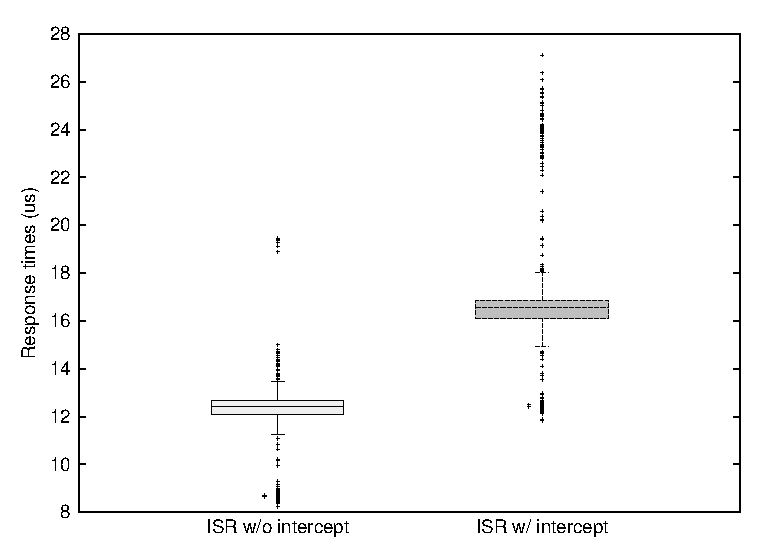
\includegraphics[width=\hsize]{img/interrupt_response}
\caption{\scriptsize{Comparison of the response time of the interrupt processing with intercept and the interrupt processing without intercept}}
\label{fig:bottomvstasklet}
\end{center}
\end{minipage}
\begin{minipage}{0.33\hsize}
\begin{center}
\includegraphics[width=0.33\hsize]{img/tasklet_vs_interrupt}
\caption{Comparison of the response time of the interrupt top-half and bottom-half}
\label{fig:bottomvstasklet}
\end{center}
\end{minipage}
\end{figure*}
\fi


\begin{figure}[t]
\begin{center}
\includegraphics[width=0.4\textwidth]{img/interrupt}
\caption{Interrupt intercept overhead}
\label{fig:irq_overhead}
\end{center}
\end{figure}
\begin{figure}[t]
\begin{center}
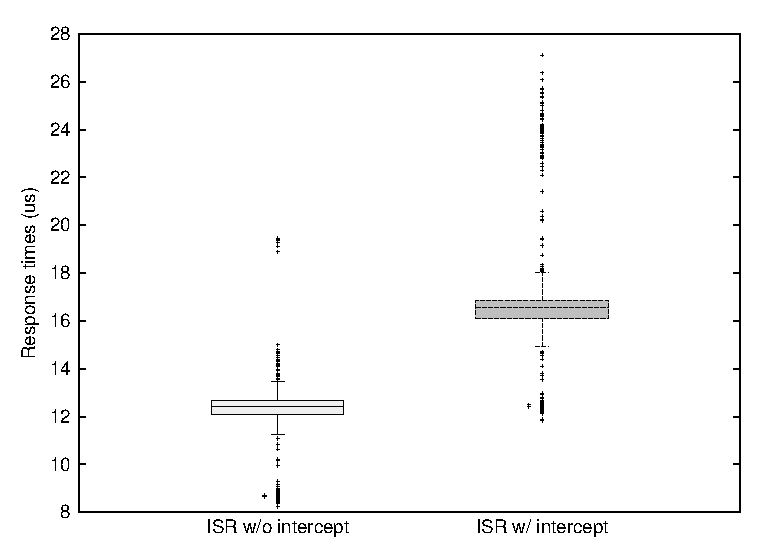
\includegraphics[width=0.4\textwidth]{img/interrupt_response}
\caption{Comparison of the response time of the interrupt processing with intercept and the interrupt processing without intercept}
\label{fig:response}
\end{center}
\end{figure}
\begin{figure}[t]
\begin{center}
\includegraphics[width=0.4\textwidth]{img/tasklet_vs_interrupt}
\caption{Comparison of the response time of the interrupt top-half and bottom-half}
\label{fig:bottomvstasklet}
\end{center}
\end{figure}

Figure~\ref{fig:irq_overhead} shows results of measurements in the above setting.
%Figure \ref{irq_overhead}は上記設定で測定した結果である。
Raw ISR is execute ISR in the original routine.
ISR Intercept is only intercept our approach.
ISR Intecept w/Func is interception with processing functions which are identify the ISR and wake-up the scheduler thread.
They are showed the average times of 1000 times with error bar is indicate minimum and maximum.

As a result, the overhead exist certainly.
ISR Intercept has overhead which is 247 nano seconds, and its overhead is 0.8\% of the entire Raw ISR process.
ISR Intercept w/Func also has overhead that is 790 nano seconds, and its overhead is 2.6\% of the entire Raw ISR process.
Intuitively, these overhead does not affect system since very small values,
however, interrupt is occur frequently including such as timer interrupt, should be aware as disadvantages.

Next, we compare response times as the interrupt impact of the interrupt itnercept.
The response times are consumption times from start interrupt processing to processing for the type.
We show the response times that are a ISR with intercept and a ISR without intercept, as a result show in Figure~\ref{fig:response}.
If we use the interrupt interception, response time become about 1.4 times as compared to without intterupt interception.
However, we targetting systems do not use the GPU runtime's resource management features.
Therefore, We should aim to fast response time of intercepted ISR, and original ISR response time is slow there is not affected much.

In addition, we evaluate comparing response time of the ISR (top-half) and the tasklet (bottom-half) in an environment with non CPU load for comparing prior works approach.
GPUSync intercept the $tasklet\_schedule()$ if $tasklet\_schedule()$ is called from the Nvidia driver.
We confirm whether the fast response time of a tasklet intercept using GPUSync and the ISR intercept.
This evaluation does measurement time until the responsible timing from the start of interrupt process which is $do\_IRQ$ function is called).
Figure~\ref{fig:bottomvstasklet} shows the result of this evaluation.
Tasklet interception response time is worse than ISR, as shown in Figure~\ref{fig:bottomvstasklet}.
This result because the tasklet is generally called after the significant procesing in ISR.

%%TODO なぜ

%Raw ISRは通常のルーチンで実行されるISR、ISR Interceptは割り込みを盗聴するのみ、
%ISR intercept w/Funcは盗聴した上でその割り込みが、いずれのカーネルに関連した割込みか識別しスケジューラを立ち上げる機能を実行した場合である。
%それぞれ1000回の測定で平均値を取り、最小値と最大値についてエラーバーで示している。
%この図から見て取れるように、オーバヘッドは確実に存在する。
%ISR Interceptだと247nsのオーバヘッドであり、
%ISR Intercept w/Funcでも790nsのオーバヘッドである。
%この数値は直感的に考えると小さくシステム自体に影響を及ぼすほどではないと考えられ、
%しかしその割込みが乱発することによる積み重ねによっては影響を与えることは、
%本手法のデメリットとして意識しなければならない。

\subsection{Independent Synchronization mechanism overhead}
We evaluated the overhead according to using the independent synchronization mechanism.
The mechanism is needed to call the $rtx\_nvrm\_notify()$ at the timing of requested synchronization (e.g. after the kernel launch issue) and $rtx\_nvrm\_init()$.
%本稿では同期生成のためのオーバヘッドを測定する。
%割込みの立ち上げは同期を求めるタイミング(e.g. カーネルラウンチ後)にrtx\_nvrm\_notify()を呼び出す必要がある。
In vanilla environment, the APIs are not necessary.
Therefore, the overhead includes the API execution time.
%スケジューリングを行わないVanillaな状態ではこれらのAPIは必要ではないものであるため、これらのAPIにかかった時間はすべてオーバヘッドとなる。
We measured the overhead by measuring API execution time between call and return of APIs.
%そのためこれらのオーバヘッドの計測を行う。計測はAPIの呼び出しから戻るまでを測定する。

\begin{figure}[!t]
\begin{center}
\subfigure[Part of Initialize]{\includegraphics[width=0.23\textwidth]{img/irq_rise_init.eps}}\subfigure[Part of notify]{\includegraphics[width=0.22\textwidth]{img/irq_rise_notify.eps}}
\caption{Interrupt raised method overhead}
\label{fig:irq_rise_overhead}
\end{center}
\end{figure}

Figure~\ref{fig:irq_rise_overhead} shows measurement result.
Initialize is need to called the at awaken a Linux process for allocating an indirect buffer and registers several engines such as compute and copy to the device driver.
Notify and Fence are GPU commands sending to GPU devices which called at timing of the need to synchronization such as after the kernel launch issues.
Execution time of the methods have scatter that is affected by ioctl system call.
%結果をFigure \ref{fig:irq_rise_overhead}に示す。
%InitializeはIndirect Bufferはプロセスが立ち上がるたびに、
%コマンド送信用のIndirect Bufferの確保や各エンジンの登録のために呼び出される必要がある。
%Notifyはカーネル実行後や非同期メモリコピー実行後のような同期を発生させたいタイミングで呼び出される。
%これらはioctlシステムコールによってユーザ空間とカーネル空間をまたいでる影響か、実行時間のバラ付きが大きく出ている。

Initialize average time is about 4msec.
However, application is not affected too much because above characteristics is only called once.
%Initializeは比較的時間がかかっているが、1プロセスにつき一度しか呼ばれないため、アプリケーション全体への影響は少ないと考えられる。
Notify is not taking much time that is about 3.5µsec.
Fence likewise is not taking much time that is about 2µsec.
Although may be not have to worry about for most applications.
However, overhead is necessary to considered in a cycle of short application.


\subsection{Scheduling Overhead}\label{sec:eval:sched_overhead}

\if 0
\begin{figure}[t]
\begin{center}
\includegraphics[width=1.5\textwidth]{img/sum_task_fp.eps}
\caption{Scheduling overhead(between GPU kernel launch request and synchronization)}
\label{fig:fp_overhead}
\end{center}
\end{figure}
\fi

\begin{figure}[t]
\begin{center}
\includegraphics[width=.44\textwidth]{img/sum_task.eps}
\caption{Scheduling overhead (Time of entire task)}
\label{fig:fp_task_overhead}
\end{center}
\end{figure}

We evaluated scheduling overhead by using the Linux-RTXG scheduler.
We prepared three applications that are ``vanilla'', ``mutex'', and ``rtx'' for measurement overheads.
These applications are based common application based on Gdev's microbenchmark which has GPU looping function.
%details
Changes are arranged to generate multiple GPU tasks by the fork.
Each tasks have 10 jobs, and a job is included GPU data transferring and a GPU kernel execution.

The ``rtx'' application is scheduled by rtx.
The ``mutex'' application  is limited to single kernel issue similar to scheduling environment.
The ``vanilla'' application is not to change the base application.

CPU scheduling policy is using the simple fixed-priority scheduling by Linux-RTXG similar to Linux's $SCHED\_FIFO$ that difference is the presence or absence of the job management.
GPU scheduling policy is fixed-priority scheduling with resrouce reservation which is BAND scheduling policy.
The synchronization is using NOTIFY of the independent synchronization mechanism.

We measured the average time in 100 times GPU task execution (1000 jobs).
The result show in Figure~\ref{fig:fp_task_overhead}.
%Figure~\ref{fig:fp_overhead} is each APIs execution average time.
%Figure~\ref{fig:fp_task_overhead} is tasks execution average time.
%計測結果をFigure~\ref{fig:fp_overhead}に示す。
%アプリケーションに含まれるタスク数ごとにプロットしており、各ジョブ内のラウンチ要求から実行完了までにかかった時間の平均値を各処理毎に積み上げ式で示している。
The ``launch\_advice'' is time of until GPU kernel launch request is accept on the Linux-RTXG.
The ``mutex'' is time to get the mutex lock.
The ``sync'' is time of untile synchronizationed from issued the GPU kernel launch issue.

Overhead increases in proportion as the number of tasks increases because task scheduling processing times is increased.
Max overhead is 10\% at the eight tasks based on "vanilla" time.
The most factors contained in the overhead is the API's overheads and scheduling algorithms (e.g. Band scheduling include yield times).
If application periods is short, users are conscious of the overheads.

%launch\_adviceはrtx\_gpu\_launchによってGPU利用のためのリクエストを出してから、許可がでるまでを示しており、
%get\_mutexはmutexによってロックを獲得するまでの時間、
%launch、notifyはそれぞれコマンドを発行するまでにかかった時間で、
%syncは発行されてから同期完了するまでの時間である。
%全て、100回のアプリケーション実行($number of tasks ☓$)の平均値である.

%rtxでスケジューリングした場合のオーバヘッドを測定するために、"vanilla", "mutex", "rtx"の3種類のアプリケーションを用意した。
%全てに共通するのが、1個のアプリケーションに複数のタスクが存在しており、
%各タスクには10個のジョブが含まれることである。1個のジョブはGPUへのデータ転送、GPUカーネル実行、GPUからのデータ転送を含んでいる。GPUカーネルは単純な行列の計算を行う。
%
%3種で異なる点として、まずmutexは同時にlaunchが発行されるのが1つに調停されるようにmutexを用いてロックしたバージョンである。
%そしてrtxはlinxu-rtxgを用いて実行したケースであり、
%vanillaはそれらの追加が無くスケジューリングや調停を一切行わないケースである。


%CPUのスケジューリングはlinux-rtxを用いたシンプルなFixed-priorityスケジューリング (LinuxのSCHED\_FIFOと同様のポリシー、ジョブ管理のみを行う)を用いる。
%GPU側のスケジューリングは、Gdevで提案されたBANDスケジューラ、Linux-RTXでの同期は全てNOTIFYを用いて行う。


\subsection{Performance of QoS management}
Next experiments are evaluating QoS management performance.
In this evaluate, we measure the utilization of each tasks on the several environments.
Thereby, we indicates performance that is not falling by not modificate kernel.
%次にGPUのバジェットエンフォースメントの性能を評価する。
%ach tasks assigned to VGPU one by one, and each VGPU is provided a GPU resource 25\%.
\begin{figure}[!t]
\begin{center}
\subfigure[FIFO Scheduling]{\includegraphics[width=0.4\textwidth]{img/fifo_rtx_nvidia}} 
\label{fig:fifo_rtx_nvidia} \\
\subfigure[BAND Scheduling]{\includegraphics[width=0.4\textwidth]{img/band_rtx_nvidia}}
\label{fig:band_rtx_nvidia}
\caption{Utilization of two tasks on the Linux RTXG scheudler and using Nvidia driver. Each tasks have different workloads and different resources (VGPU0 = 40\%, VGPU1 = 60\%).}
\label{fig:rtx_nvidia}
\end{center}
\end{figure}

\begin{figure}[!t]
\begin{center}
\subfigure[FIFO Scheduling]{\includegraphics[width=0.4\textwidth]{img/fifo_rtx}}
\label{fig:fifo_rtx} \\
\subfigure[BAND Scheduling]{\includegraphics[width=0.4\textwidth]{img/band_rtx}}
\label{fig:band_rtx}
\caption{Utilization of two tasks on the Linux RTXG scheudler and using Nouveau driver. Each tasks have different workloads and different resources (VGPU0 = 40\%, VGPU1 = 60\%).}
\label{fig:rtx_nouveau}
\end{center}
\end{figure}

\begin{figure}[t]
\begin{center}
\includegraphics[width=0.5\textwidth]{img/band_rtx_fair}
\caption{Utilization of four tasks on the Linux-RTXG's BAND VGPU scheduling. Each tasks have a fair workload and a fair resources.}
\label{fig:band_rtx_fair}
\end{center}
\end{figure}

\if 0
\begin{figure}[t]
\begin{center}
\includegraphics[width=0.5\textwidth]{img/band_rtx_diff}
\caption{Utilization of four tasks on the Linux-RTXG's BAND VGPU scheduling. Each tasks have a different workload and a different resources.}
\end{center}
\label{fig:band_rtx}
\end{figure}
\fi

\if 0
\begin{figure}[t]
\begin{center}
\includegraphics[width=0.5\textwidth]{img/dummy}
\caption{Utilization of four tasks on the G. All tasks are fairy given resources which is 25\%}
\end{center}
\label{fig:qos_gdev}
\end{figure}
\fi

We experiment task isolation performances on the Linux-RTXG's GPU scheduler with GPU driver which is used the Nvidia GPU driver and the Nouveau GPU driver.
The first, we measure the utilization of the running two GPU tasks.
The each GPU tasks have a different workload and a different resource.
A GPU task is allocated VGPU0, and given the 40\% resource, and has about 1.2 times the workload of other tasks.
The other GPU task is allocated VGPU1, and given the 60\% resource.
VGPU1's task is to start after about 5 seconds of VGPU0's task.

A Nvidia GPU driver's result is showed in Figures~\ref{fig:rtx_nvidia}.
The FIFO scheduling policies shown in Figure~\ref{fig:rtx_nvidia}(a),
and the BAND scheduling policies~\cite{kato:gdev} shown in Figure~\ref{fig:rtx_nvidia}(b).
A Nouveau GPU driver's result is showed in Figures~\ref{fig:rtx_nouveau}.
The FIFO scheduling policies shown in Figure~\ref{fig:rtx_nouveau}(a),
and the BAND scheduling policies shown in Figure~\ref{fig:rtx_nouveau}(b).
Figure~\ref{fig:rtx_nvidia}(a),~\ref{fig:rtx_nouveau}(a) indicate that the GPU tasks performed in accordance with the workload by fair scheduling.
On the other hand, Figure~\ref{fig:rtx_nvidia}(b),~\ref{fig:rtx_nouveau}(b) indicate that the GPU tasks performed in accordance with the utilization by resource reservation mechanisms.
A VGPU1's maximum error is about 3\% in the starting BAND scheduling policies resource management using by Nvidia GPU driver, and a VGPU0's maximum error is about 5\%.
A VGPU1's maximum error is about 2\% in the starting BAND scheduling policies resource management using by Nouveau GPU driver, and a VGPU0's maximum error is about 2\%.
Large spikes are occured by GPU kernel's overrun.
If the GPU scheduler need to large spike is reduced, the GPU scheduler is needed to runtime approachs such as making preemptive GPU kernel.

The second, we measure the utilization of the running four GPU tasks.
The each GPU tasks have a same workload and same resources, and each GPU tasks allocate to each VGPUs.
The BAND scheduling policies result shown in Figure~\ref{fig:band_rtx_fair}.
A maximum error of these VGPUs is about 9\%, it values are happend by a timing of budget replenish and a synchronization latency.  
%the variance of Gdev is \textbf{x}.
%We can be seen that the performance is not nearly falling from the above results
%Linux−RTXGの振幅は◯%以下であり,Nouveauの振幅は◯%以下である.
%Linux-RTXGの分散は◯であり,Nouveauの分散は◯なことから,性能はほぼ落ちていないことがわかる.
%最後に非周期タスクが存在する環境下においても,QoS Managementによってリソース制限がかかっていることを示すことで,
Therefore, the synchronization mechanism of Linux-RTXG excluding kernel modification is show that possible scheduling without sacrificing performance.

%つまり,Linux-RTXGのカーネル編集を除いたシンクロナイゼーションメカニズムにおいても,
%性能を落とさずにスケジューリング可能なことを示せている.



%ここでは、今回同一アルゴリズムでQoSマネージメントを行っているGdevとの比較を行い、
%パッチを利用しない実装においても、性能をほぼ落とすこと無くできていることを示す。

%比較対象は、本Linux-RTXGと同様のスケジューリングアルゴリズムが提供可能なGdevのモジュール版とで比較する。
%評価に用いるスケジューリングポリシーはBANDスケジューラを用いる。
%実験に利用するアプリケーションとして、\ref{sec:eval:sched_overhead}節で利用したものと同様のものでTaskを4つ生成し、各タスク毎に25\%のGPU利用権限を与える。
%これらのタスクの実行中のGPU利用率を計測し、Gdevと同様のアルゴリズムを用いることで、今回提供するLinux−RTXGによるアプローチによってどれだけQoSマネージメントについてのパフォーマンスに影響するかを示す。
%Gdevを用いることから、両者ともデバイスドライバはNouveauドライバを用いる.
